%!TEX root = ../dissertation.tex


\chapter{\label{chap:halo}Neutrino Halo Problem}


One of the big questions about neutrino oscillations in supernovae is the so called halo problem. Cherry et al showed that neutrino flavor conversions are greatly affected by the back scattered neutrinos in supernovae~\cite{Cherry2012}. Neutrinos around supernovae are scattered and some of them are scattered to move almost backward. On the other hand, neutrino self-interactions is proportional to the inner product of momenta of neutrinos, which leads to the dependence on $1-\cos\theta$ where $\theta$ is the angles between momenta of two neutrinos. Most of the research has been concentrating on mostly forward scattering, with small values for $1-\cos\theta$. For back ward scattered neutrinos, the interaction potential can be much larger than the forward scattered neutrino contributions. Though the work by Sarikas et al showed that matter suppression is still significant within this region~\cite{Sarikas2012a}, it is not clear how exactly the neutrino halo alters neutrino oscillations. The halo problem itself is worth more calculations. In this chapter, I will present a relaxation method for this problem. The focus will be on the numerical method itself.


\section{\label{chap:halo-sec:line}Line Model}

We continue to use the simplified line model and build our intuitions out of it. The halo problem is simplified to have neutrinos emitted from a line $z=0$ homogeneously, which are reflected from a certain distance $z=L$. In principle, the reflection angles doesn’t have to be Snell’s law. The scattering can be in any angle with different amplitudes. Here I am using this very simple Snell’s law just to explore the effect of halo. It's crucial to keep an eye on the simplifications in this line model.
\begin{itemize}
    \item Neutrinos are emitted from a line, which is not the case in a real supernova.
    \item Neutrinos are emitted with translation symmetry on the line. Breaking the symmetry might bring in other qualitatively different results.
    \item Neutrinos are reflected from a certain surface $z=L$, which is different from reality where neutrinos are scattered everywhere.
    \item Neutrinos are reflected according to Snell's law.
    \item Neutrinos are homogeneously reflected at $z=L$.
\end{itemize}



\begin{figure}
    \centering
    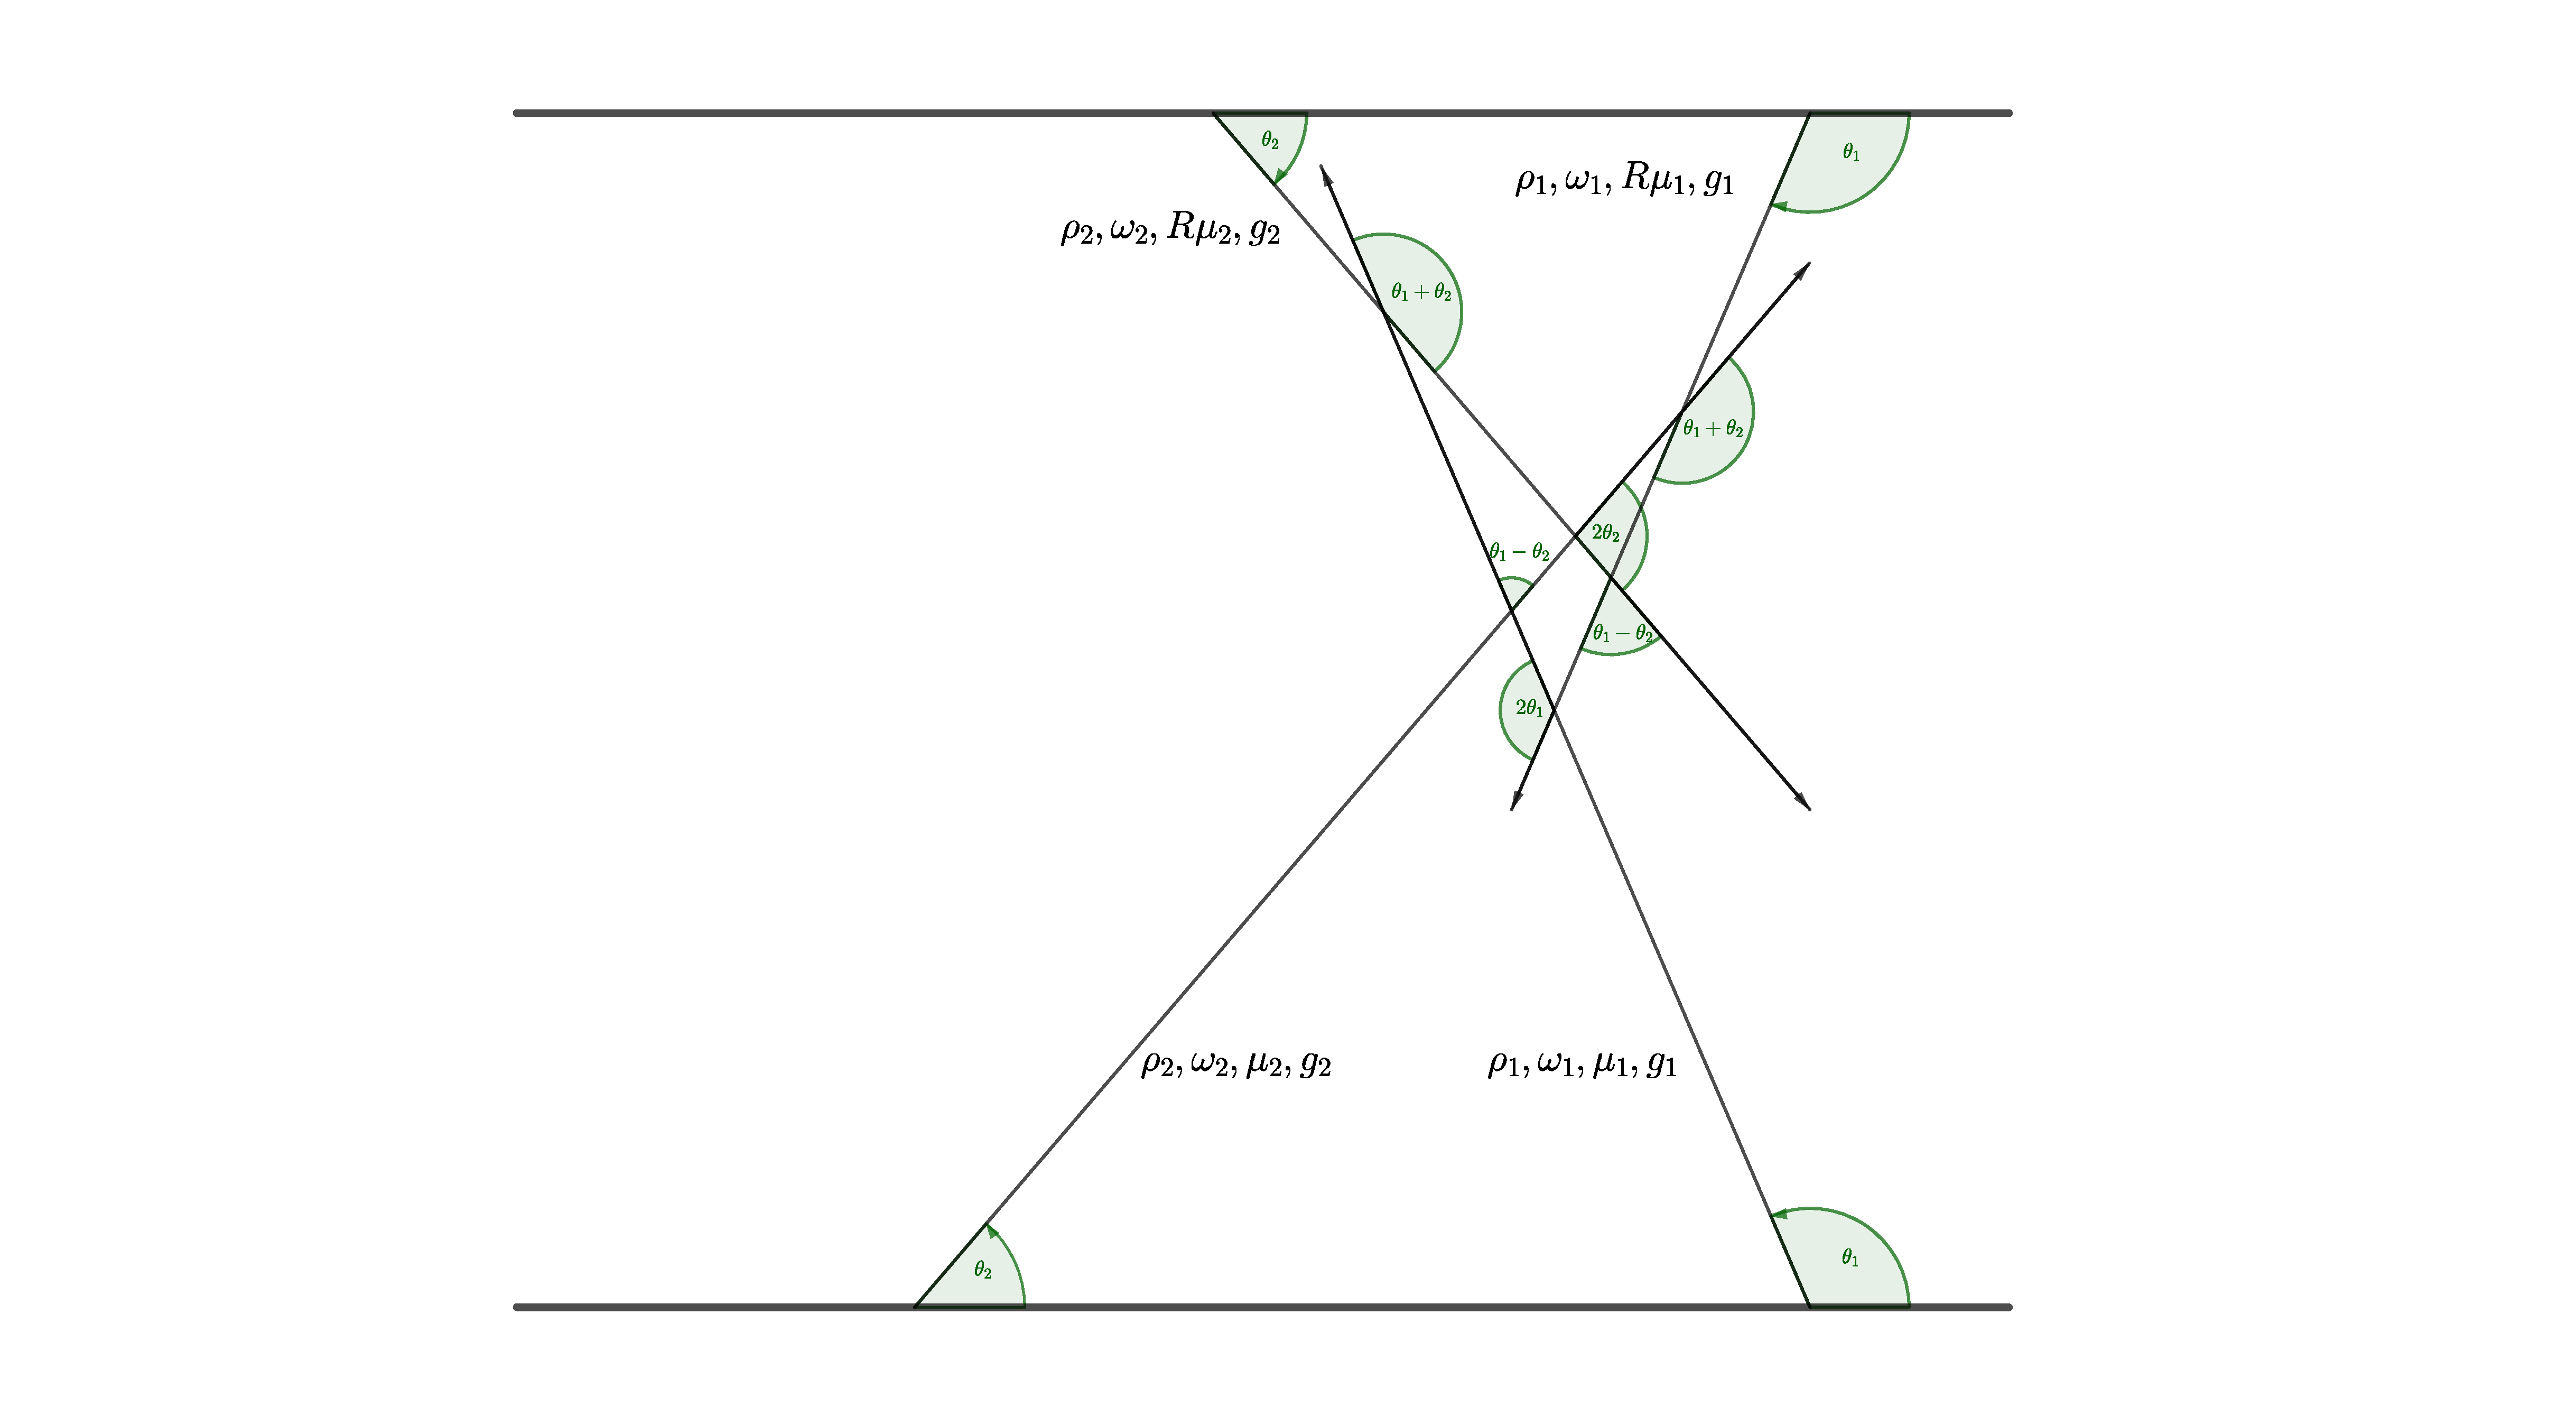
\includegraphics[width=\textwidth]{chapters/assets/halo/line-model.pdf}
    \caption{Line model used for halo problem. Neutrinos are emitted from the bottom line and reflected at the top line.}
    \label{chap:halo-sec:line-fig:line-model}
\end{figure}


The algorithm that I used is relaxation method. The algorithm is meant to find the equilibrium state of neutrino oscillations with the presence of halo.
\begin{enumerate}
\item Calculate forward beam using 0 backward beam;
\item Calculate backward beam using forward beam calculated in 1;
\item Calculate forward beam using backward beam calculated in 2;
\item Repeat until the beams reach equilibrium.
\end{enumerate}


\section{\label{chap:halo-sec:line-sym}Neutrino Beams Only}

As a first step, I calculated neutrino oscillations with only neutrino beams. Before we rush to the numerical results, I linearized the equation of motion and worked out the linear stability analysis.

In linear regime, we define the density matrices for forward and backward beams to be
\begin{align*}
   \rho_F &= \frac{1}{2} \begin{pmatrix}
   1 & \epsilon_F \\
   \epsilon_B^* & -1
   \end{pmatrix} \\
   \rho_B &= \frac{1}{2} \begin{pmatrix}
   1 & \epsilon_B \\
   \epsilon_B^* & -1
   \end{pmatrix}.
\end{align*}
The Hamiltonian for forward and back ward beams are
\begin{align*}
   H_F &= H_v + R \mu \rho_B \\
   H_B &= H_v + \mu \rho_F.
\end{align*}
We will investigate the instability for zero mixing angle for new instabilities. The linearized equation of motion can be simplified to
\begin{align*}
   i\partial_z \begin{pmatrix}
   \epsilon_F \\
   \epsilon_B
   \end{pmatrix} = \begin{pmatrix}
   -\omega_v + R \xi \mu & - R \xi \mu \\
   \xi \mu & \omega_v - \xi \mu
   \end{pmatrix} \begin{pmatrix}
   \epsilon_F \\
   \epsilon_B
   \end{pmatrix}.
\end{align*}
This equation can be easily solved. The eigenvalues are
\begin{align*}
   \Omega_+ &= \frac{1}{2} ( (R-1)\xi\mu + \sqrt{\Delta} ) \\
   \Omega_- &= \frac{1}{2} ( (R-1)\xi\mu - \sqrt{\Delta} ),
\end{align*}
where
\begin{equation}
   \Delta = (1-R)^2 \mu^2 \xi^2 - 4\mu\xi \omega_v (1+R) + 4\omega_v^2.
\end{equation}
The corresponding eigenvectors are
\begin{align*}
   V_+ &=\begin{pmatrix}
   \frac{ -2\omega_v + \xi \mu (1+R) + \sqrt{\Delta} }{2\xi\mu} \\
   1
   \end{pmatrix} \\
   V_- &=\begin{pmatrix}
   \frac{ -2\omega_v + \xi \mu (1+R) - \sqrt{\Delta} }{2\xi\mu} \\
   1
   \end{pmatrix}.
\end{align*}
The general solution to the equation is
\begin{equation*}
   \begin{pmatrix}
   \epsilon_F(z) \\
   \epsilon_B(z)
   \end{pmatrix} = C_+ V_+ e^{-i \Omega_+ z} +  C_- V_- e^{-i \Omega_- z}.
\end{equation*}

The special property about this reflection problem is that the density matrices for the forward and backward beams should be the same at the reflection point, say $z=L$. With such a simple relation, we can find the relations between $C_\pm$ by setting $\epsilon_F(L)=\epsilon_B(L)$,
\begin{equation}
   \frac{C_+}{C_-} = e^{-i(\Omega_- -\Omega_+)L} \frac{ \sqrt{\Delta} +  2\omega_v + \mu \xi (1-R) }{\sqrt{\Delta} -  2\omega_v - \mu \xi (1-R)}.
\end{equation}
The solution to be problem can be simplified,
\begin{equation}
   \begin{pmatrix}
   \epsilon_F(z) \\
   \epsilon_B(z)
   \end{pmatrix} = C_- e^{-i\Omega_- L} \left( \frac{ \sqrt{\Delta} +  2\omega_v + \mu \xi (1-R) }{\sqrt{\Delta} -  2\omega_v - \mu \xi (1-R)} V_+ e^{-i \Omega_+ (z-L)} +  V_- e^{-i \Omega_- (z-L)} \right).
\end{equation}

We are interested in the absolute values of each elements so that the overall factors can be neglected. The forward beam evolution is obtained by taking the absolute value of $\epsilon_F$,
\begin{align*}
   \left\vert \epsilon_F \right\vert \propto & \lvert (2\omega_v +\xi\mu(1-R) +i \delta ) ( -2\omega_v + \xi\mu(1+R) + i \delta ) e^{\delta(z-L)} \\ 
   &+ ( -2\omega_v - \xi\mu(1-R) +i \delta ) ( -2\omega_v + \xi\mu(1+R) - i \delta ) e^{-\delta(z-L)} \rvert,
\end{align*}
in which $\sqrt{\Delta}$ is replaced by $i \delta$. We collecting terms and verify that it has the form
\begin{equation}
   \left\vert \epsilon_F \right\vert \propto A + B \cosh( 2\delta(L-z) ),
\end{equation}
where $B\leq 0$.
The only $z$ dependent term is $\cosh( 2\delta(L-z) )$, which is decreasing within $[0,L]$ and is increasing in $[L,2L]$. The slope at $z=L$ is 0. An example is plotted in Fig.~\ref{chap:halo-sec:line-sym-fig:cosh}.


\begin{figure}[!htbp]
    \centering
    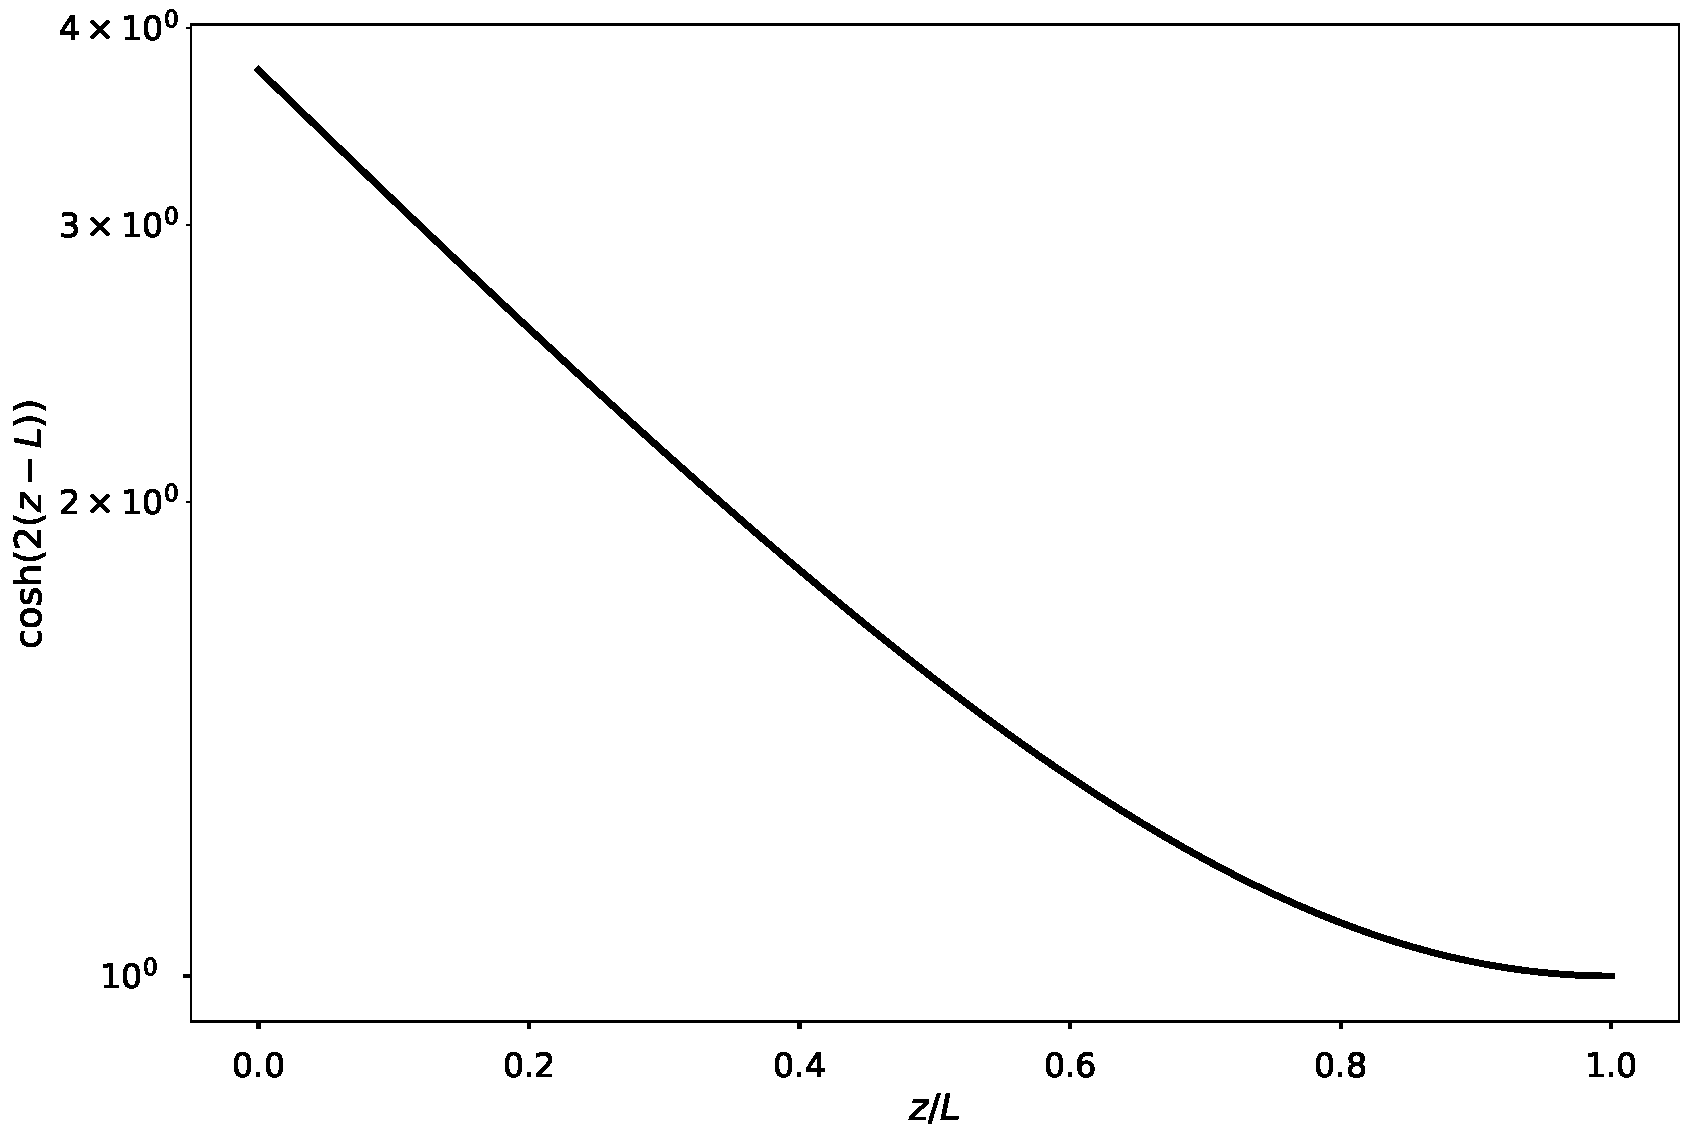
\includegraphics[width=\textwidth]{chapters/assets/halo/cosh.pdf}
    \caption{ An example of $\cosh(2\delta(z-L))$ with $\delta=1$, and $L=5$.}
    \label{chap:halo-sec:line-sym-fig:cosh}
\end{figure}


We expect the numerical calculations bare the same behavior that the instability leads to no growth but decrease in flavor conversion, assuming the neutrinos start from electron flavor. The result indeed confirms it. Fig.~\ref{chap:halo-sec:line-sym-fig:mu-1.0-reflection-0.07} is an example of it.

\begin{figure}[htbp]
    \centering
    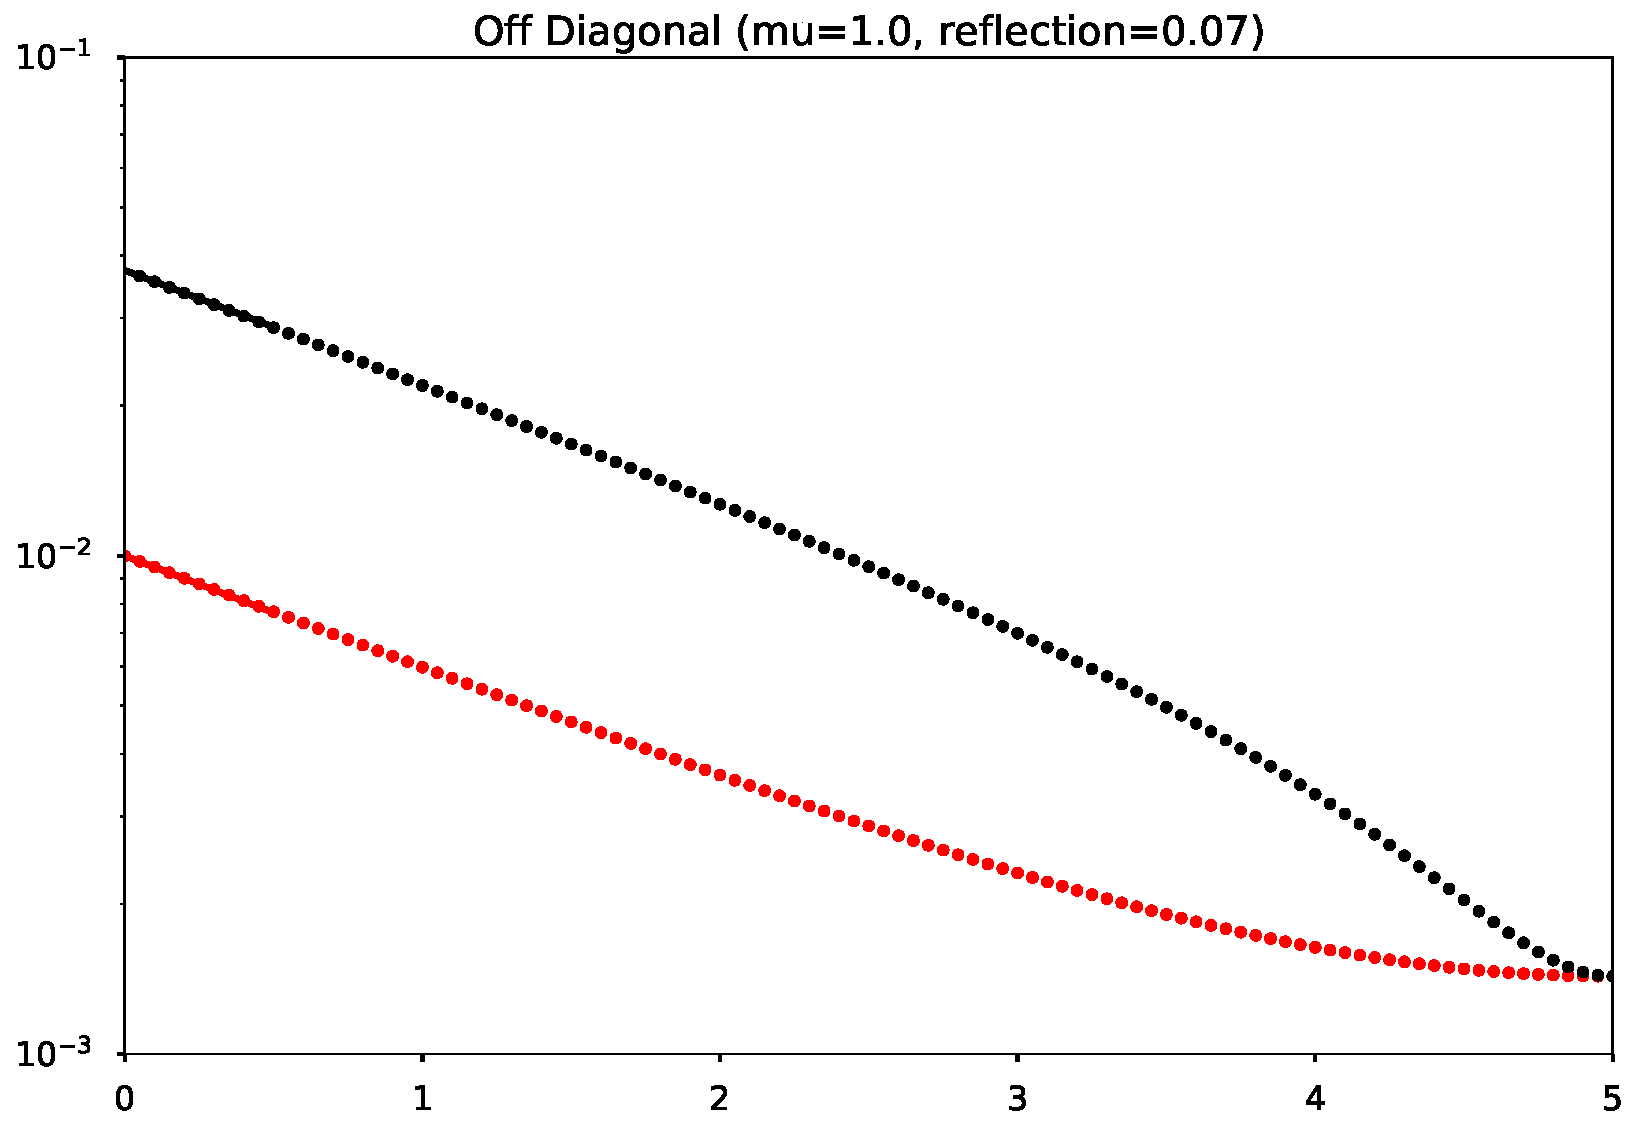
\includegraphics[width=\textwidth]{chapters/assets/halo/mu-1-reflection-0p07.pdf}
    \caption{Absolute value of off diagonal element for $\mu=1.0$, $R=0.07$, $L=5$, with normal hierarchy. The red dots are for the forward beam and the black dots are for the backward beams. The lines are indicating the predictions of linear stability analysis.}
    \label{chap:halo-sec:line-sym-fig:mu-1.0-reflection-0.07}
\end{figure}

For linear stability analysis, we usually identify real characteristic values of the linearized equation of motion. In bipolar model as explained in Sec.~\ref{chap:app-sec:bipolar}, real characteristic values of the equation of motion indicates exponential growth, while it always indicates exponential decrease in this simplified halo problem. 

We expect that only normal hierarchy has an instability region which is trivial since we noticed that the backward beam is acting like antineutrino beams but with different hierarchies.
\begin{align}
 i \partial_t \mathbf s_F &= \mathbf s_F \times (\mathbf {H}_v +R \mu \mathbf s_B) \\
   i\partial_t \mathbf s_B &= \mathbf s_B \times (- \mathbf H_v - \mu \mathbf s_F) .
\end{align}
Compare to Eq.~\ref{chap:app-sec:bipolar-eqn:flavor-isospin-eom}, we notice that 
the reflected beam works as an antineutrino beam but the system becomes the opposite hierarchy compared to bipolar model. We find the instability regions in Fig.~\ref{chap:halo-sec:line-sym-fig:instability-regions}.


\begin{figure}[htbp]
    % \centering
    \minipage{0.49\textwidth}
    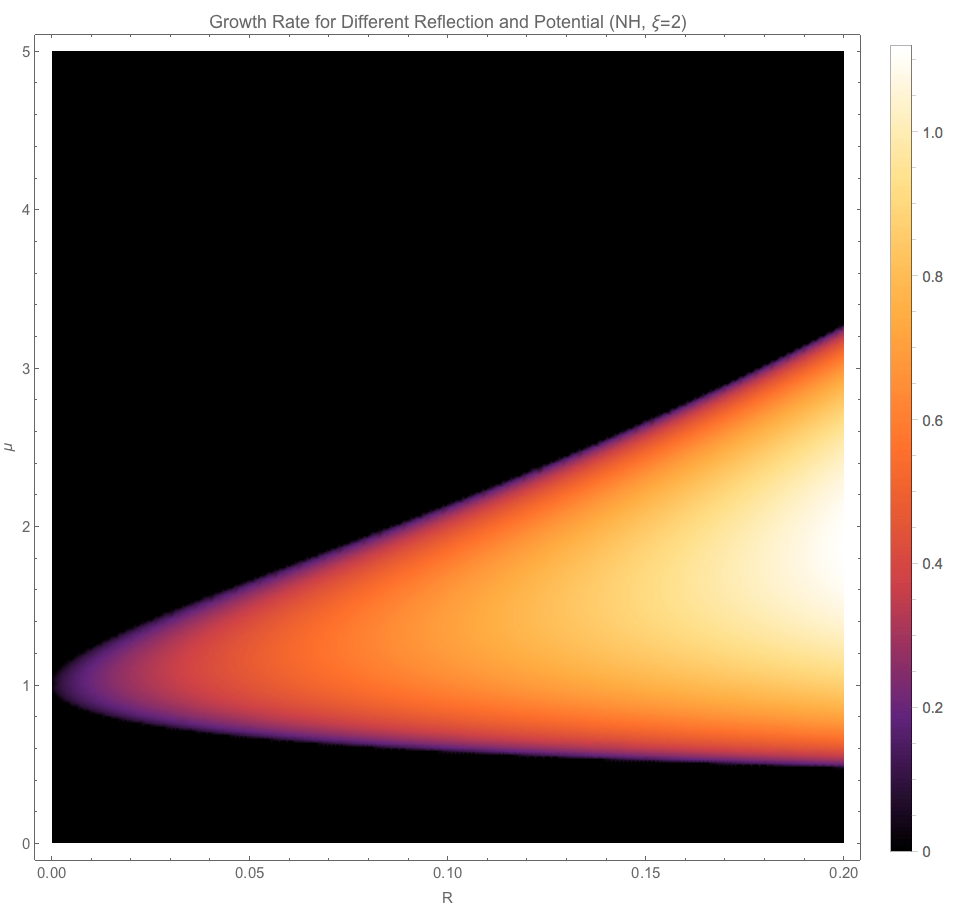
\includegraphics[width=\textwidth]{chapters/assets/halo/growth-rate-mu-refl-nh.jpg}
    \endminipage\hfill
    \minipage{0.49\textwidth}
    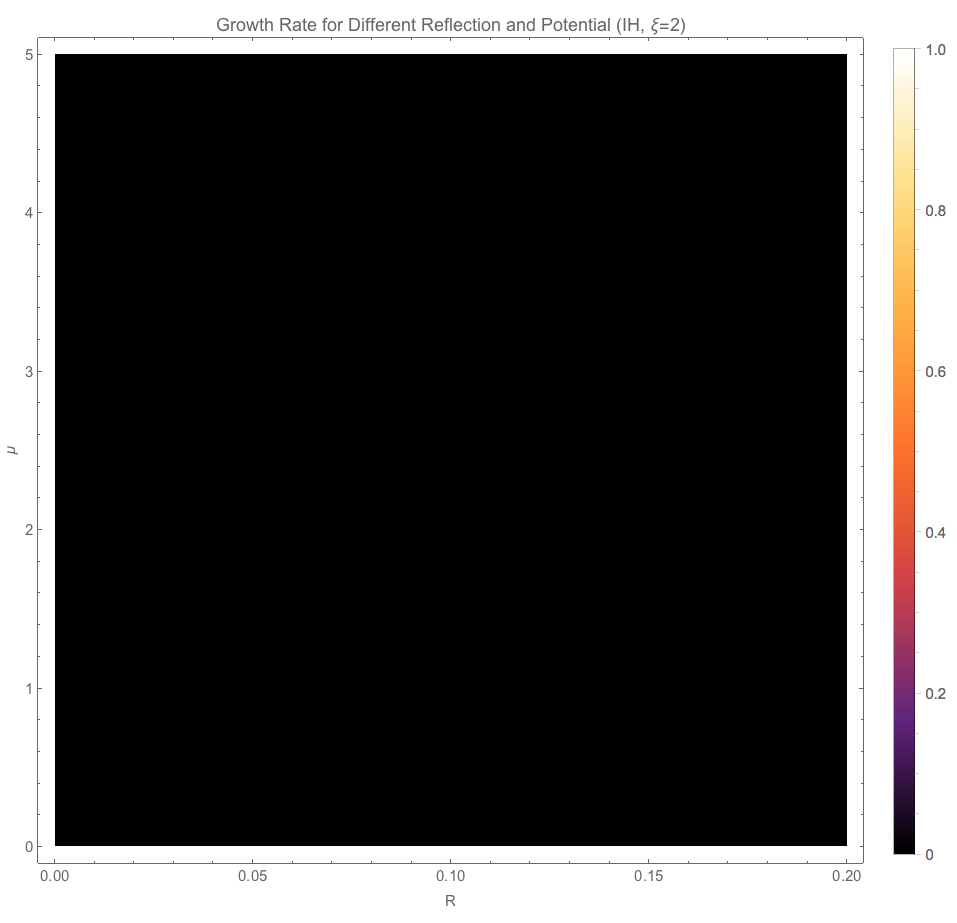
\includegraphics[width=\textwidth]{chapters/assets/halo/growth-rate-mu-refl-ih.jpg}
    \endminipage\hfill
    \caption{Instability regions for normal hierarchy (left) and inverted hierarchy (right) as a function of neutrino potential $\mu$ and reflection coefficient $R$, with vacuum mixing angle set to 0.}
    \label{chap:halo-sec:line-sym-fig:instability-regions}
\end{figure}




\section{Two Beams Model with Reflection}

The model is naturally extended to a two beams model including both neutrinos and antineutrinos. The configuration is exactly the same as shown in Fig.~\ref{chap:halo-sec:line-fig:line-model}.

As the first step we work out the linear stability analysis. The four equations of motion are
\begin{align}
    i \partial_z \rho_1 = & [ H_1, \rho_1 ], \\
    i \partial_z \rho_2 = & [ H_2, \rho_2 ], \\
    -i \partial_z \rho_3 = & [ H_3, \rho_3 ], \\
    -i \partial_z \rho_4 = & [ H_4, \rho_4 ],
\end{align}
where ${}_1$ and ${}_2$ are the quantities for two forward beams while ${}_3$ and ${}_4$ are the quantities for the corresponding backward going beams. For the purpose of this analysis we set $\theta_v = 0$. The Hamiltonians are
\begin{align}
    H_1 =& -\eta \omega_v \sigma_3 + g_2 \chi_- \mu_2 \rho_2 + g_2 \chi_+ R \mu_2 \rho_4 + g_1 \chi_1 R \mu_1 \rho_3, \\
    H_2 =& \eta \omega_v \sigma_3 + g_1 \chi_- \mu_1 \rho_1 + g_2 \chi_2 R \mu_2 \rho_4 + g_1 \chi_+ R \mu_1 \rho_3, \\
    H_3 =& -\eta \omega_v \sigma_3 + R g_2 \chi_- \mu_2 \rho_4 + g_2 \chi_+\mu_2 \rho_2 + g_1 \chi_1 \mu_1 \rho_1, \\
    H_4 =& \eta \omega_v \sigma_3 + R g_1 \mu_1 \chi_- \rho_3 + g_1 \chi_+ \mu_1 \rho_1 + g_2 \chi_2 \mu_2 \rho_2.
\end{align}

I have defined 
\begin{align*}
    \chi_+ = & 1 - \cos ( \theta_1 + \theta_2 ), \\
    \chi_- = & 1 - \cos ( \theta_1 - \theta_2 ), \\
    \chi_1 = & 1 - \cos ( 2\theta_1 ), \\
    \chi_2 = & 1 - \cos ( 2\theta_2 ),
\end{align*}
and $g_i$ represents the energy spectrum of the neutrinos and $\eta$ stands for the hierarchy.

% Linear stability analysis can be done using computer.

\section{\label{chap:halo-sec:num}Relaxation Method for Numerical Solutions}


We choose a relaxation method scheme to solve this non-local boundary value problem numerically. To begin with, we write down the discretization scheme.
\begin{align}
    \rho(t+\Delta t) &= \left[  \cos( 2 h \Delta t)\rho_n -  2 u_i \rho_i u_n \right]\sigma_n \\
    &= \left[  \cos( 2 h \Delta t) \rho_n +  2 \sin^2(h \Delta t) u'_i \rho_i u'_n \right]\sigma_n
\end{align}
The reason that we use fixed step size for this problem is that it's easier to calculate the neutrino self-interactions on such fixed grids. The algorithm is described as
\begin{enumerate}
    \item
Calculate forward beam using 0 backward beam;
\item
Calculate backward beam and forward beam together using the state of beams from the previous step current counter beams;
\item
Repeat the previous step until the state of the beams reach equilibrium.
\end{enumerate}
To speed up the calculations, I also implemented OpenMP for parallel computing. The code is tested using vacuum oscillations (shown in Fig.~\ref{chap:halo-sec:num-fig:compare-vac-bipolar}) and bipolar models. The reason that we still have conversions is because of the vacuum term, which is additional to linear stability analysis. It is also proven to reach equilibrium quickly as shown in Fig.~\ref{chap:halo-sec:num-fig:relax-color}. 

\begin{figure}
    \minipage{0.49\textwidth}
    % 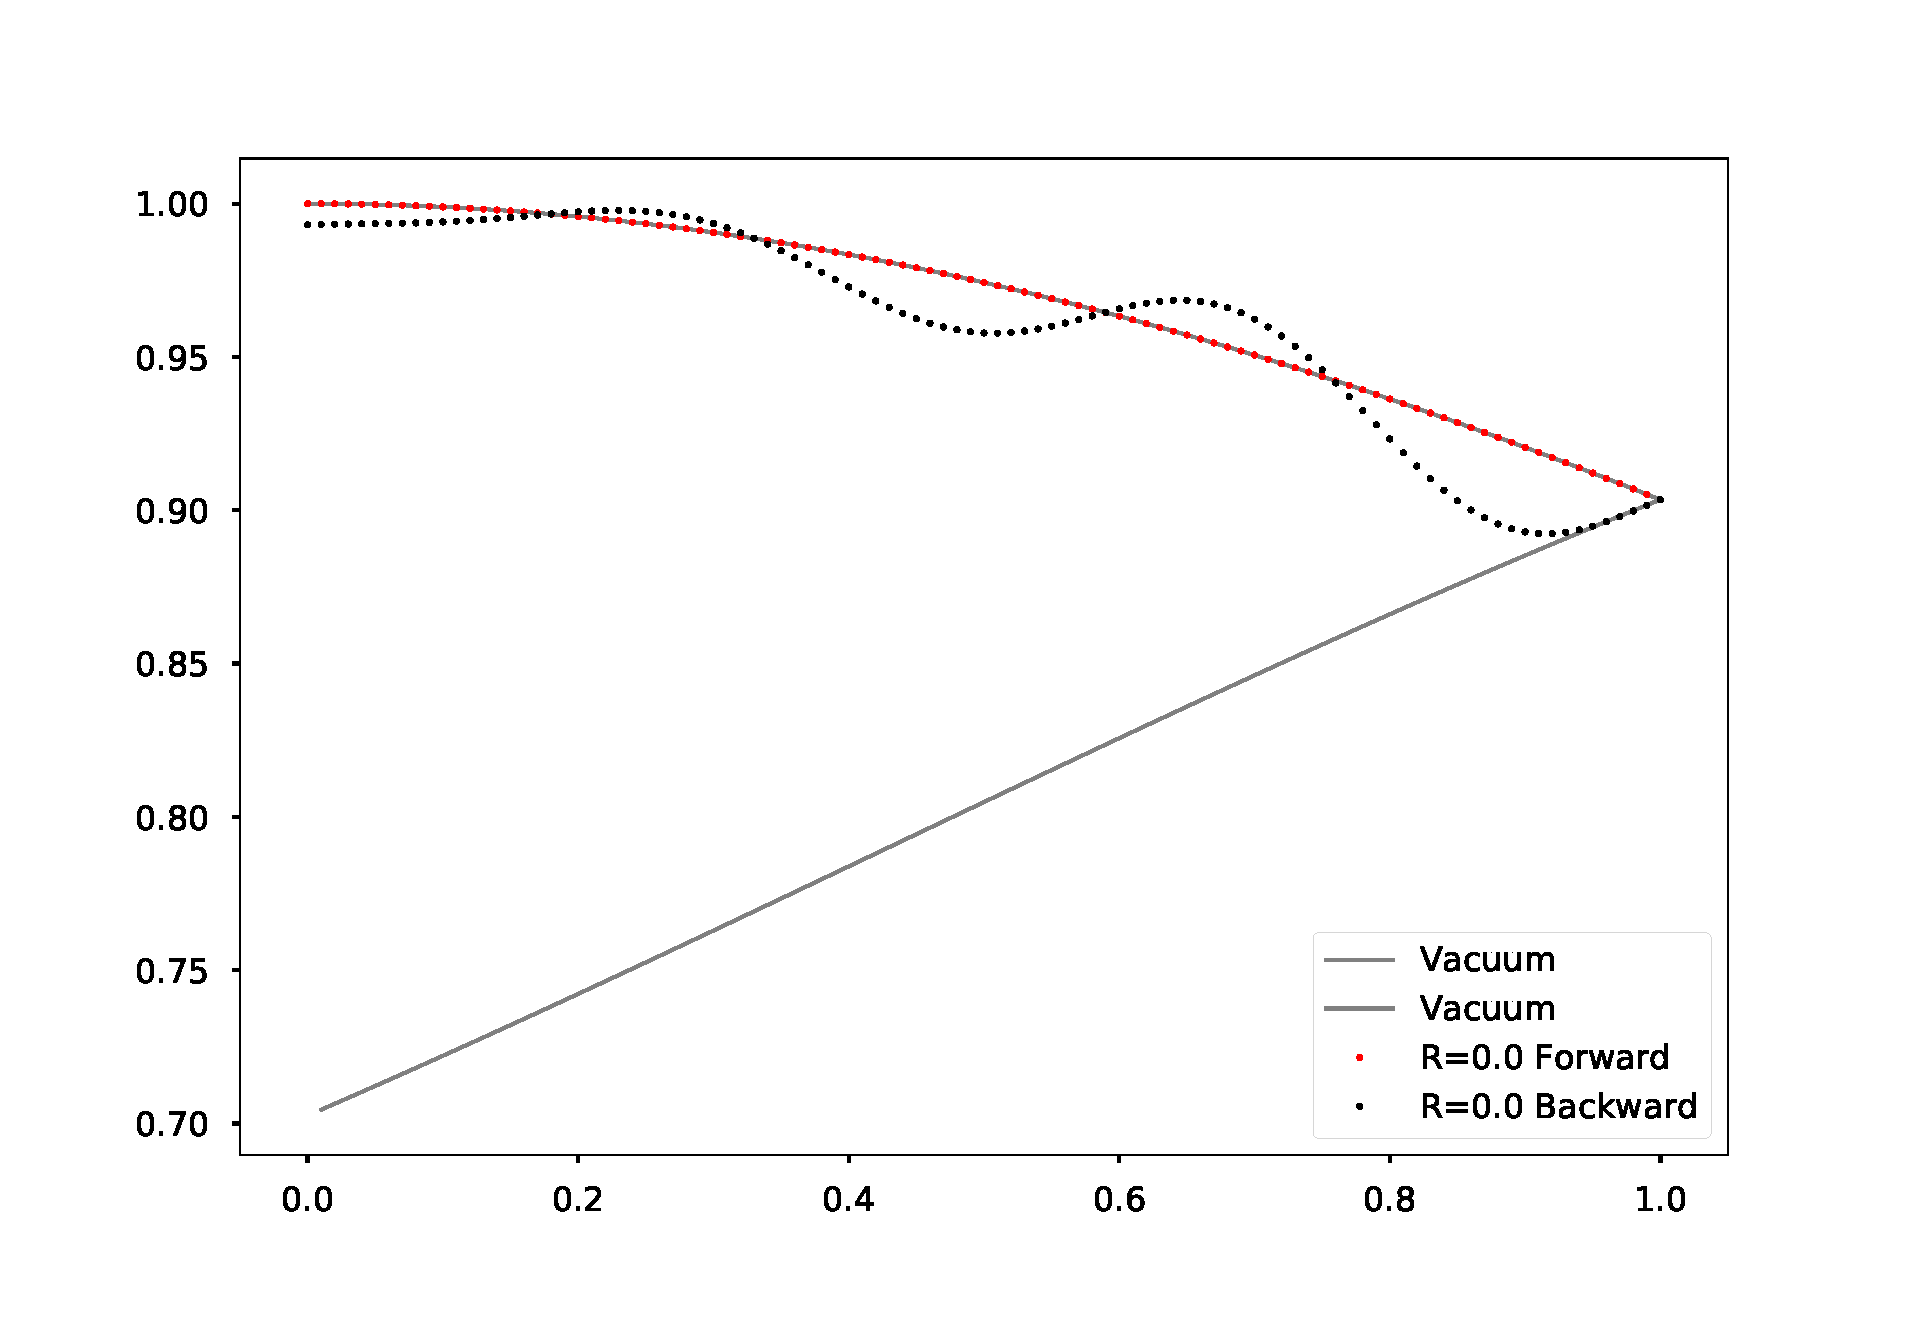
\includegraphics[width=\textwidth]{chapters/assets/halo/halo-mu-4-compare-vac.pdf}
    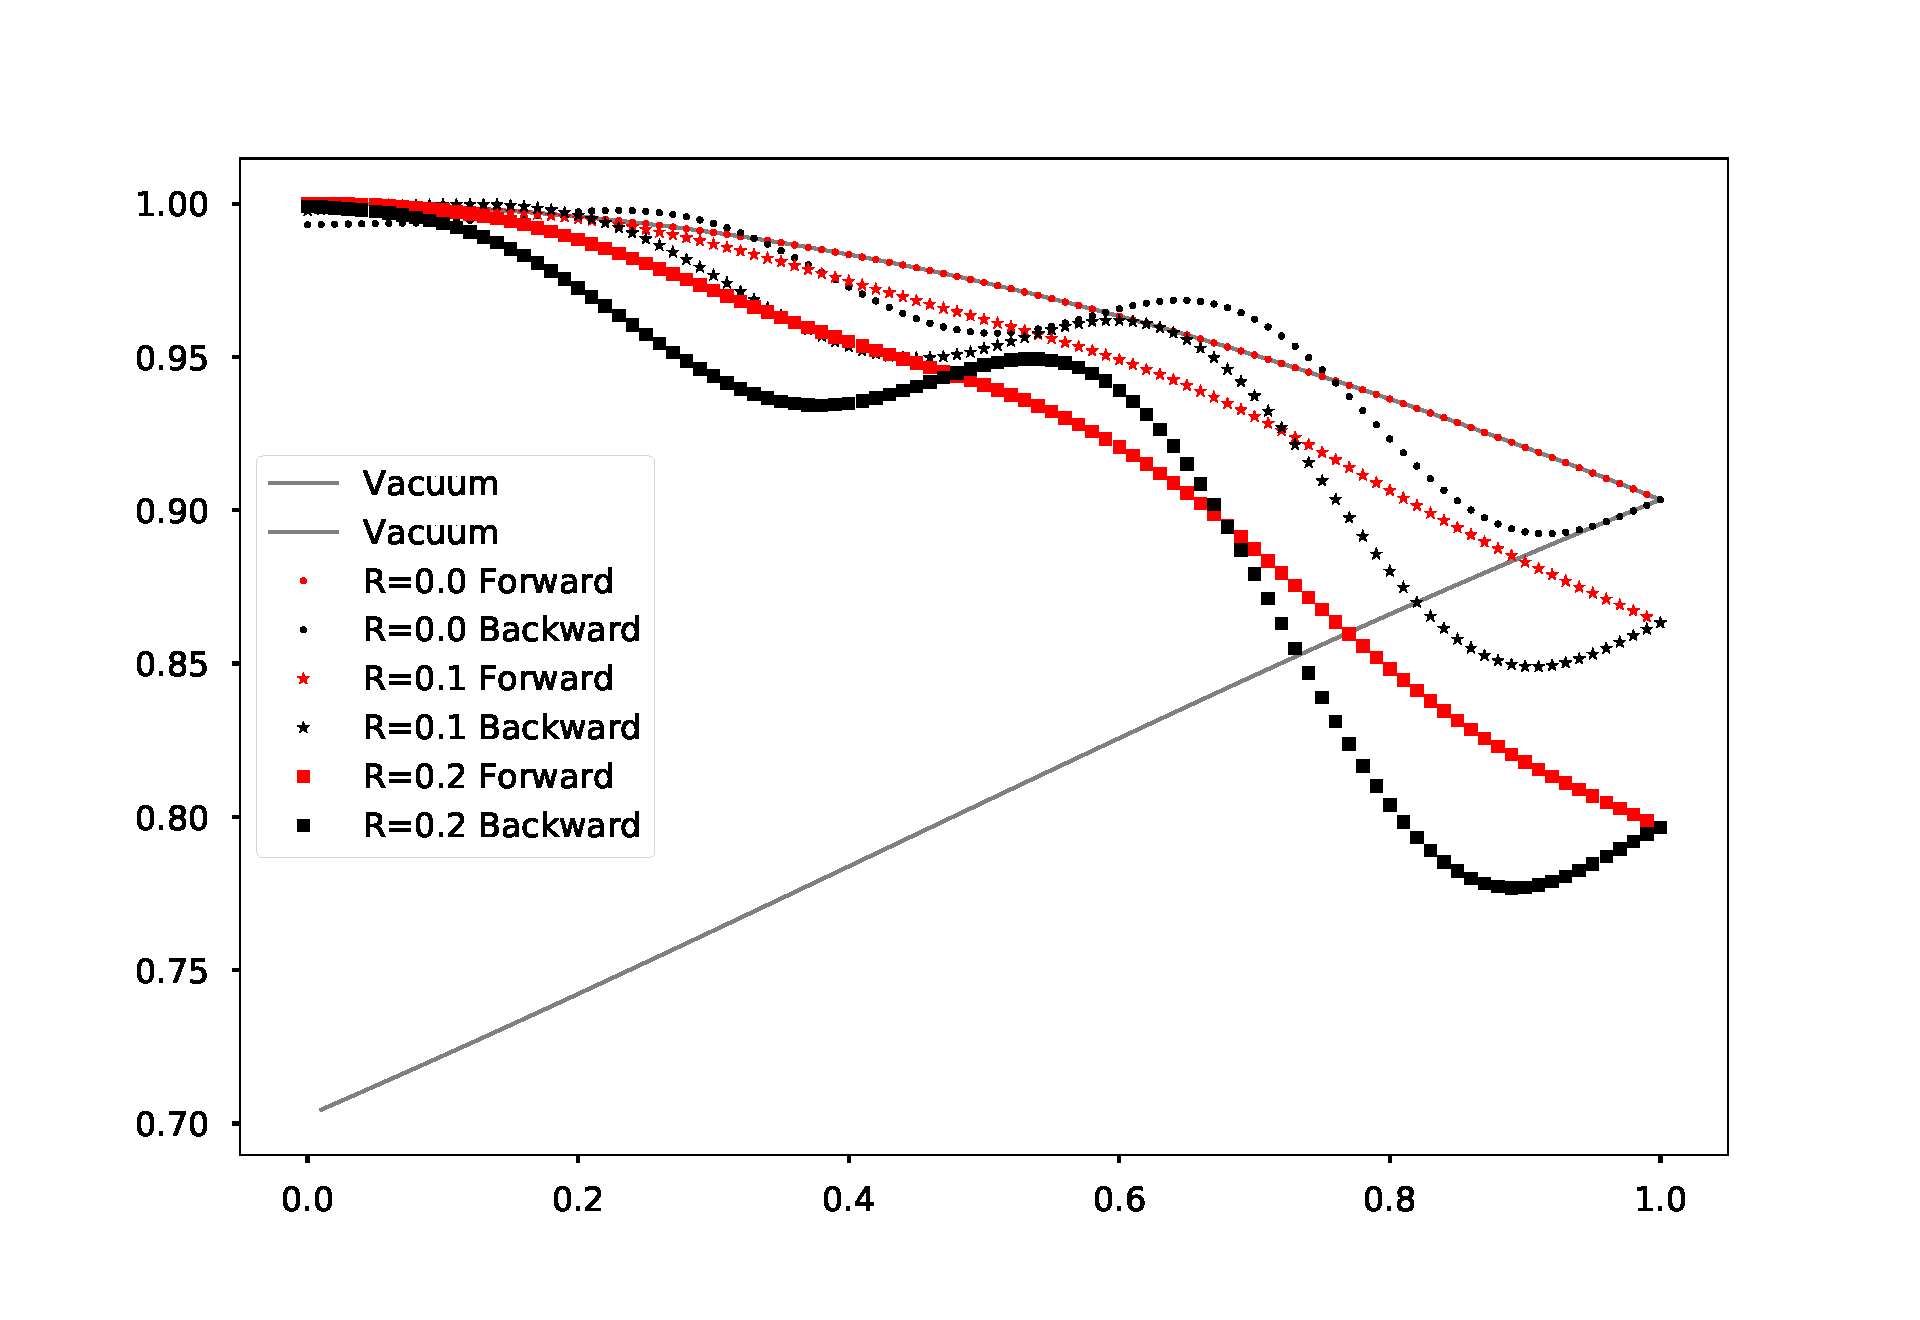
\includegraphics[width=\textwidth]{chapters/assets/halo/halo-mu-4-r-multiple.pdf}
    \endminipage\hfill
    \minipage{0.49\textwidth}
    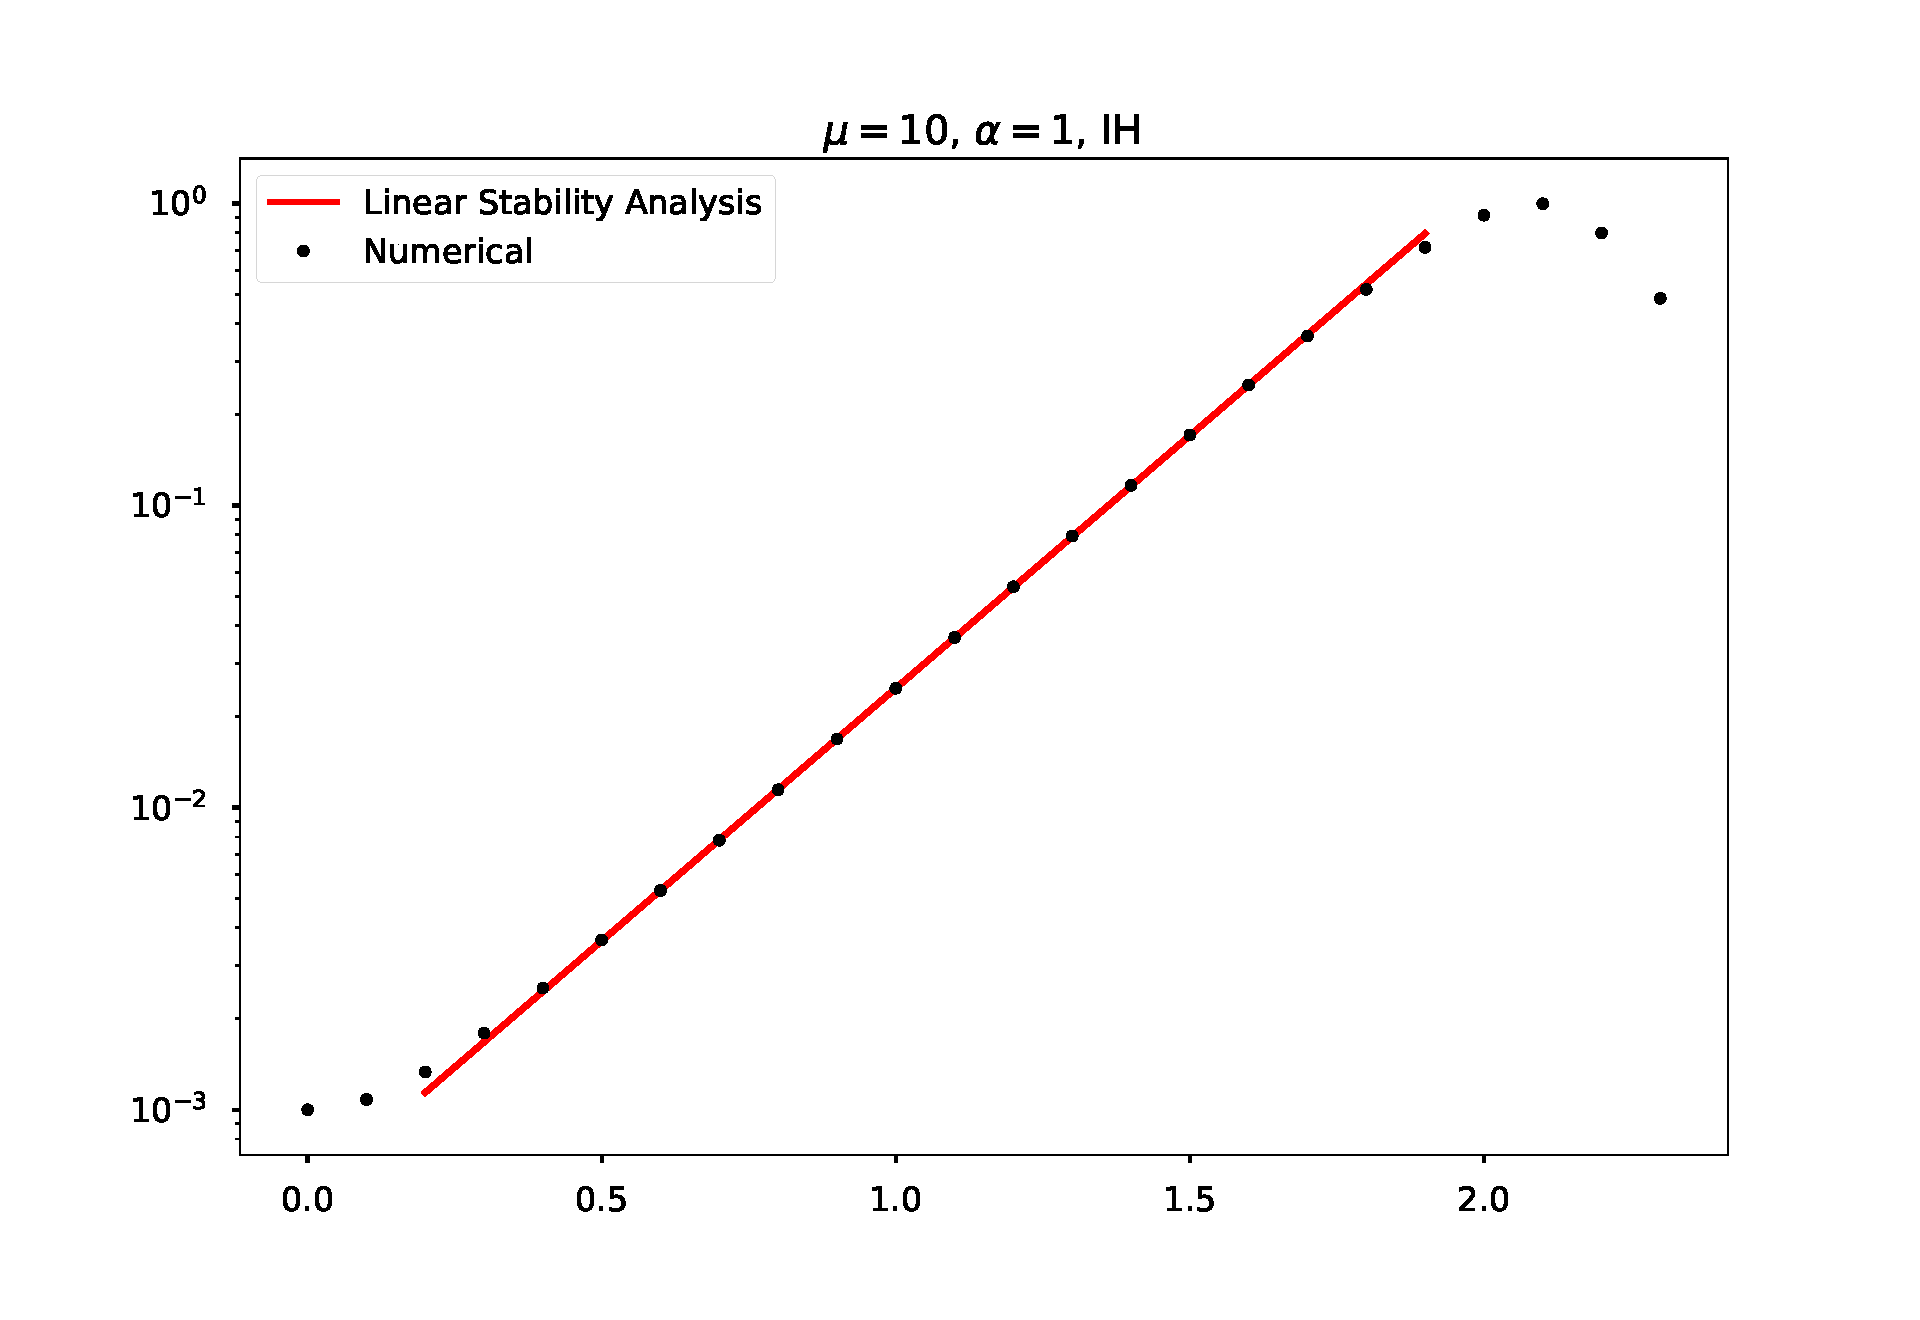
\includegraphics[width=\textwidth]{chapters/assets/halo/halo-mu-4-compare-bipolar.pdf}
    \endminipage\hfill
    \caption{The left panel validates code by setting reflection to zero and approach vacuum for single forward beam. Meanwhile, we notice that for nonzero reflections, more conversion is done, which makes sense due to the similarity between $R$ and the asymmetry parameter $\alpha$ in bipolar model. The right panel validates the code by setting reflection to zero and compare with bipolar model for two beams case, where the slope matching the theoretical value $3.85$.}
    \label{chap:halo-sec:num-fig:compare-vac-bipolar}
\end{figure}

\begin{figure}
    \centering
    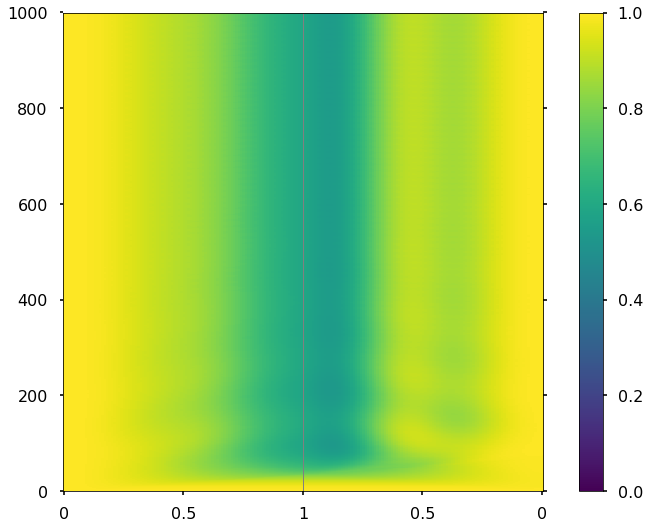
\includegraphics[width=\textwidth]{chapters/assets/halo/relax-color.png}
    \caption{Relaxation method reach equilibrium after some steps. This calculation sets $\mu = 4$, $R=0.2$, and is done within range $[0,1]$.}
    \label{chap:halo-sec:num-fig:relax-color}
\end{figure}





\section{Conclusion}

Halo problem brings in more parameters to neutrino oscillations. In the spirit of numerical methods, we developed a parallelable relaxation method, using C++ and OpenMP. Both the analytical and numerical results showed that for the two realms, either single forward beam or two forward beams, we spot trivial results by drawing analogy with bipolar model, alas no new types of instabilities was found in these situations. On the other hand, reflection indeed may enhance the flavor conversions. Future work should be done to explore the effect of symmetry breakings in the problem.